\documentclass[addressstd,a4paper,10pt]{dinbrief}

\usepackage[spanish,activeacute]{babel}
\usepackage[T1]{fontenc}
\usepackage[ansinew]{inputenc}
\usepackage{lmodern} %Type1-font for non-english texts and characters

%% Packages for Graphics & Figures %%%%%%%%%%%%%%%%%%%%%%%%%%
\usepackage{graphicx} %%For loading graphic files

\usepackage{mathtools}
\usepackage{listings}
\usepackage{caption}



\usepackage{listings}
 %Type1-font for non-english texts and characters
\usepackage[scaled]{beramono}
%% Images can be included using \includegraphics{Dateiname}
%% resp. using the dialog in the Insert menu.
%% 
%% The mode "LaTeX => PDF" allows the following formats:
%%   .jpg  .png  .pdf  .mps
%% 
%% The modes "LaTeX => DVI", "LaTeX => PS" und "LaTeX => PS => PDF"
%% allow the following formats:
%%   .eps  .ps  .bmp  .pict  .pntg




%% Address of the Sender %%%%%%%%%%%%%%%%%%%%%%%%%%%%%%%%%%%%




\pagestyle{empty} %%No heads and feets



%%%%%%%%%%%%%%%%%%%%%%%%%%%%%%%%%%%%%%%%%%%%%%%%%%%%%%%%%%%%%
%% DOCUMENT - LETTER(S)
%%%%%%%%%%%%%%%%%%%%%%%%%%%%%%%%%%%%%%%%%%%%%%%%%%%%%%%%%%%%%
\begin{document}



Instituto Polit\'ecnico Nacional
\begin{lstlisting}
\end{lstlisting}
Escuela Superior de C\'omputo
\begin{lstlisting}
\end{lstlisting}
Ana Paola Nava Vivas
\begin{lstlisting}
\end{lstlisting}
2CM4

\begin{lstlisting}
\end{lstlisting}
\begin{lstlisting}
\end{lstlisting}
\begin{lstlisting}
\end{lstlisting}
\begin{lstlisting}
\end{lstlisting}
Conversi\'on de NFA a e-NFA, y de e-NFA a DFA:
\begin{lstlisting}
\end{lstlisting}
\begin{lstlisting}
\end{lstlisting}
\begin{lstlisting}
\end{lstlisting}

Aut\'omata finito no determinista, NFA:
\begin{lstlisting}
(0+1)*01
\end{lstlisting}


\begin{center}
\begin{figure}
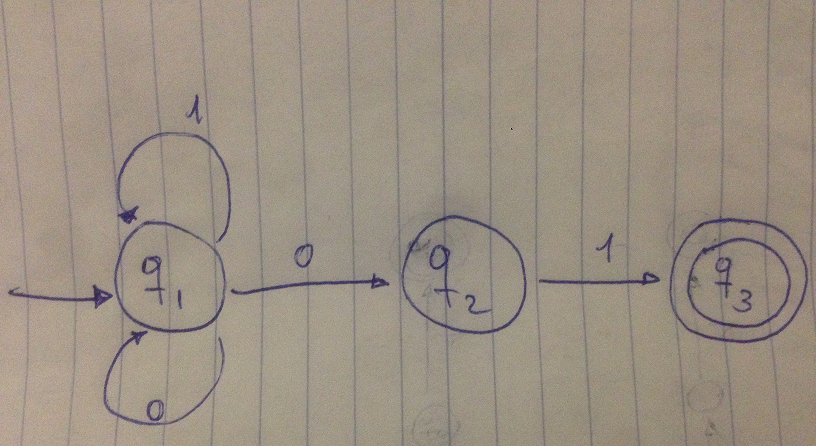
\includegraphics[width=0.9\textwidth]{NFA.png} 
\centering
\end{figure}
\end{center}

\begin{lstlisting}
\end{lstlisting}
\begin{lstlisting}
\end{lstlisting}
\begin{lstlisting}
\end{lstlisting}
\begin{lstlisting}
\end{lstlisting}
\begin{lstlisting}
\end{lstlisting}
\begin{lstlisting}
\end{lstlisting}
\begin{lstlisting}
\end{lstlisting}
\begin{lstlisting}
\end{lstlisting}
\begin{lstlisting}
\end{lstlisting}
\begin{lstlisting}
\end{lstlisting}
\begin{lstlisting}
\end{lstlisting}
\begin{lstlisting}
\end{lstlisting}
\begin{lstlisting}
\end{lstlisting}
\begin{lstlisting}
\end{lstlisting}
Aut\'omata finito no determinista, con \'epsilon (e-NFA).
\begin{lstlisting}
\end{lstlisting}

\begin{center}
\begin{figure}
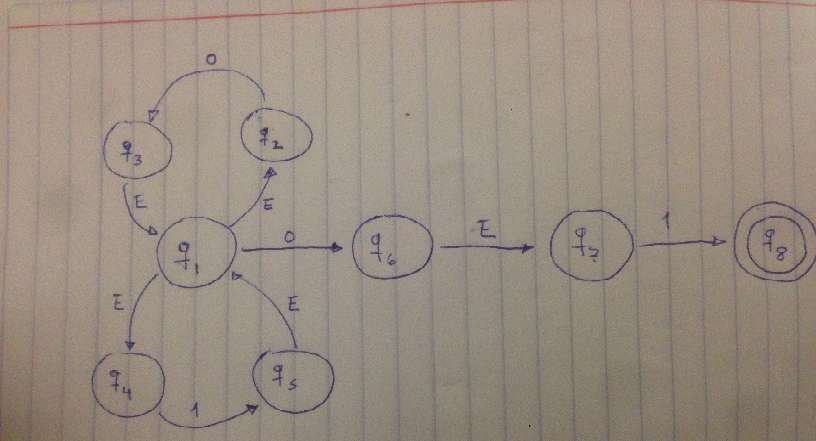
\includegraphics[width=1\textwidth]{ENFA.png} 
\centering
\end{figure}
\end{center}

\begin{lstlisting}
\end{lstlisting}
Transformaci\'on de e-NFA a DFA:
\begin{lstlisting}
\end{lstlisting}
1- Se deben encontrar las transiciones de \'epsilon para cada estado:
\begin{center}
\begin{figure}
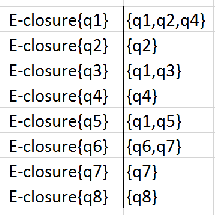
\includegraphics[width=0.6\textwidth]{eclosure.png} 
\centering
\end{figure}
\end{center}


\begin{lstlisting}
\end{lstlisting}
\begin{lstlisting}
\end{lstlisting}
\begin{lstlisting}
\end{lstlisting}
\begin{lstlisting}
.
\end{lstlisting}
2- Luego se debe dibujar la tabla de transiciones:
\end{lstlisting}
\begin{lstlisting}
\end{lstlisting}
\begin{lstlisting}
\end{lstlisting}
\begin{center}
\begin{figure}
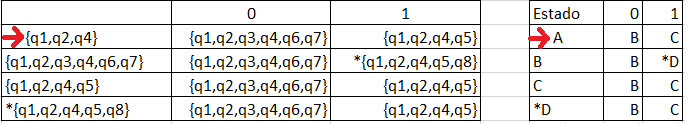
\includegraphics[width=0.9\textwidth]{tablatrans.png} 
\centering
\end{figure}
\end{center}

\begin{lstlisting}
\end{lstlisting}
\begin{lstlisting}
\end{lstlisting}
\begin{lstlisting}
\end{lstlisting}
3- Entonces ya se puede representar el aut\'omata finito determin\'istico, DFA:
\begin{lstlisting}
\end{lstlisting}
\begin{center}
\begin{figure}
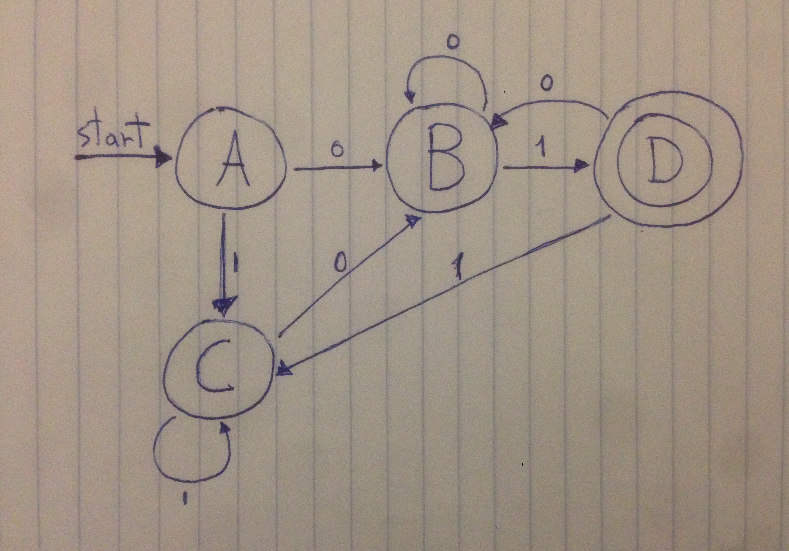
\includegraphics[width=0.9\textwidth]{DFA.png} 
\centering
\end{figure}
\end{center}




\end{document}
